\documentclass[12pt,a4paper]{article}
\usepackage[utf8]{inputenc}
\usepackage{amsmath}
\usepackage{amsfonts}
\usepackage{amssymb}
\usepackage[brazil]{babel}
\usepackage{indentfirst}
\usepackage{url}
\usepackage{listings}
\RequirePackage{graphicx}
\title{Layout responsivo / adaptivo}
\author{Andrey Silva Ribeiro \and Jeferson Rossini Ferreira Lourenço}
\usepackage[left=3cm,right=3cm,top=2cm,bottom=2cm]{geometry}

\usepackage{color}

\definecolor{mygreen}{rgb}{0,0.6,0}
\definecolor{mygray}{rgb}{0.5,0.5,0.5}
\definecolor{mymauve}{rgb}{0.58,0,0.82}

\lstset{ %
  backgroundcolor=\color{white},   % choose the background color; you must add \usepackage{color} or \usepackage{xcolor}; should come as last argument
  basicstyle=\footnotesize,        % the size of the fonts that are used for the code
  breakatwhitespace=false,         % sets if automatic breaks should only happen at whitespace
  breaklines=true,                 % sets automatic line breaking
  captionpos=b,                    % sets the caption-position to bottom
  commentstyle=\color{mygreen},    % comment style
  deletekeywords={...},            % if you want to delete keywords from the given language
  escapeinside={\%*}{*)},          % if you want to add LaTeX within your code
  extendedchars=true,              % lets you use non-ASCII characters; for 8-bits encodings only, does not work with UTF-8
  frame=single,	                   % adds a frame around the code
  keepspaces=true,                 % keeps spaces in text, useful for keeping indentation of code (possibly needs columns=flexible)
  keywordstyle=\color{blue},       % keyword style
  language=Octave,                 % the language of the code
  morekeywords={*,...},            % if you want to add more keywords to the set
  numbers=left,                    % where to put the line-numbers; possible values are (none, left, right)
  numbersep=5pt,                   % how far the line-numbers are from the code
  numberstyle=\tiny\color{mygray}, % the style that is used for the line-numbers
  rulecolor=\color{black},         % if not set, the frame-color may be changed on line-breaks within not-black text (e.g. comments (green here))
  showspaces=false,                % show spaces everywhere adding particular underscores; it overrides 'showstringspaces'
  showstringspaces=false,          % underline spaces within strings only
  showtabs=false,                  % show tabs within strings adding particular underscores
  stepnumber=2,                    % the step between two line-numbers. If it's 1, each line will be numbered
  stringstyle=\color{mymauve},     % string literal style
  tabsize=2,	                   % sets default tabsize to 2 spaces
  title=\lstname                   % show the filename of files included with \lstinputlisting; also try caption instead of title
}


\begin{document}
\begin{titlepage}


\begin{center}
\begin{figure}[htb]
		
		\label{figura:LogoIF}
	
		\centering
		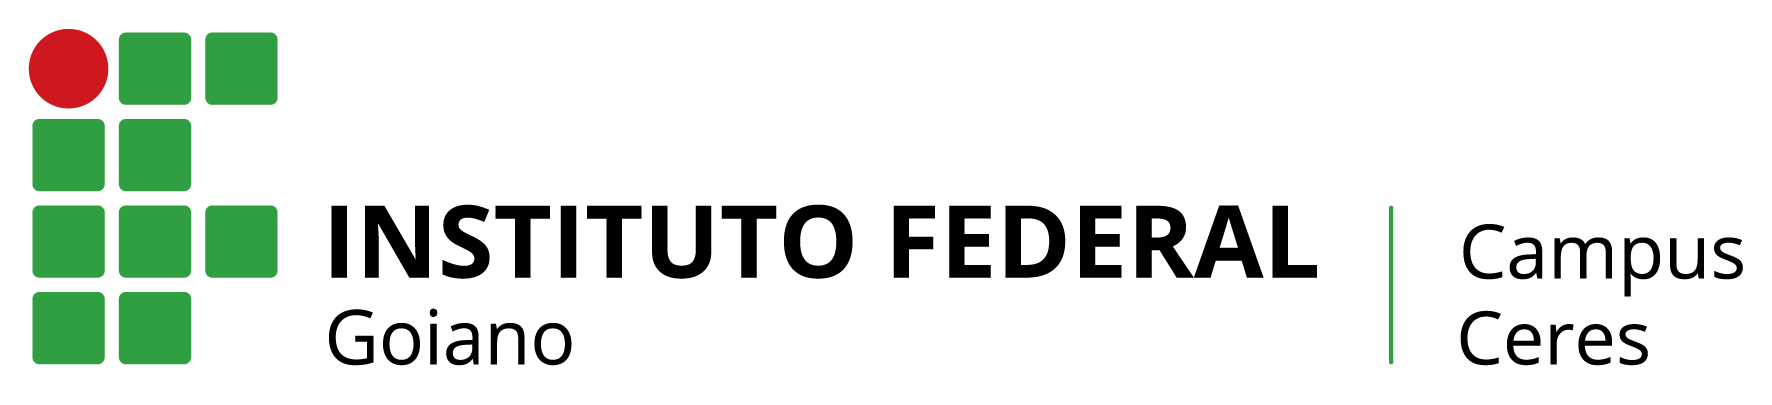
\includegraphics[width=6cm]{logo.png} 
\end{figure}


Instituto Federal Goiano - Campus Ceres\\
Bacharelado em Sistemas de Informação\\
Prof. Me. Ronneesley Moura Teles\\\vspace{0.2cm}
Andrey Silva Ribeiro \\
Jeferson Rossini Ferreira Lourenço \\

\vspace{5.0cm}

\textit{\textbf{\Large Layout responsivo / adaptivo}}\\\vspace{0.5cm}
\vspace{9.5cm}

Outubro\\
2017\\
\end{center}
\end{titlepage}



\tableofcontents

\newpage
\begin{center}
\textbf{\Large{Layout responsivo / adaptivo}}\\\vspace{0.5cm}
\end{center}

\section{Introdução}

Com o crescimento acelerado dos dispositivos móveis que navegam na internet, grande parte da Web ainda não otimizada para esses dispositivos que são limitados pelo tamanho da tela e necessitam de uma abordagem diferente para o layout.

Os tamanhos de tela mudam entre celulares, tablets, deslktops e consoles de jogos, logo é importante que seu site possa se adaptar a todos os tamanhos de telas que existem ou possam vir a existir.

\section{Responsive Web Design}
Originalmente definido por Ethan Marcotte, o Web design responsivo reage às necessidades dos usuários e seus dispositivos, mudando de acordo com o tamanho da tela e seus recursos.

Um exemplo disso é que enquanto um tablet poderia mostrar um conteúdo em duas colunas, em um celular os usuário veriam o mesmo conteúdo em uma só coluna.

Páginas que são otimizadas para reagir a diferentes dispositivos devem incluir uma tag meta viewport no cabeçalho do documento, essa tag instrui o navegador como controlar o tamanho e o dimensionamento da página.

\subsection{Tag viewport} 
\lstinputlisting{recursos/exe1.html}

Use a tag meta viewport para controlar a largura e o dimensionamento da janela de visualização dos navegadores.

Enumerando então fica:
\begin{itemize}
\item width=device-width para corresponder à largura da tela em pixels independentes de dispositivo.

\item initial-scale=1 para estabelecer uma relação 1:1 entre pixels CSS e pixels independentes de dispositivo.

\item user-scalable=no está opção impede que o usuário consiga ativar o zoom da página em smartphones. 
\end{itemize}

Tentando oferecer uma melhor experiência, navegadores móveis renderizarão a página à largura de uma tela de desktop (geralmente cerca de 980 pixels, mas isso varia de acordo com os dispositivos) e tentarão melhorar a aparência do conteúdo aumentando os tamanhos das fontes e dimensionando o conteúdo para que ele caiba na tela. Isso significa que os tamanhos das fontes podem parecer inconsistentes para os usuários, que precisarão tocar duas vezes ou controlar o zoom com gestos de pinça para ver e interagir com o conteúdo.

Usar o valor meta viewport width=device-width instrui a página a acompanhar a largura da tela em pixels independentes de dispositivos. Isso permite que a página ajuste o fluxo do conteúdo para diferentes tamanhos de telas, seja para renderização em pequenos celulares ou para um grande monitor de desktop.


\section{Já adicionei a meta no meu html, más o layout não está visivelmente elegante, e agora?
}
Consultas de mídia nos permitem criar uma experiência responsiva, onde estilos específicos são aplicados a telas pequenas, telas grades e qualquer tela intermediária. A sintaxe da consulta de mídia permite a criação de regras que podem ser aplicadas dependendo das características do dispositivo.

\subsection{Media Query} 
\lstinputlisting{recursos/exe2.html}

Embora existam vários itens para os quais possamos fazer consultas, os mais usados para um Web design responsivo são min-width, max-width, min-height e max-height.
Além disso, o uso do min-device-width pode impedir que o conteúdo se adapte em desktops ou outros dispositivos que permitam que as janelas sejam redimensionadas, pois a consulta é baseada no tamanho do dispositivo, não no da janela do navegador.

\begin{figure}[!htb]
\centering
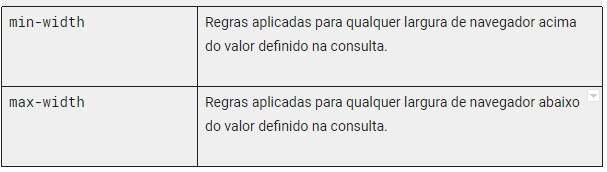
\includegraphics[width=15cm]{recursos/1.jpg}
\label{Media}
\caption{Media Query. Fonte: https://developers.google.com/web/fundamentals/design-and-ux/responsive/?hl=pt-br em 27/10/2017}
\end{figure}

\begin{figure}[!htb]
\centering
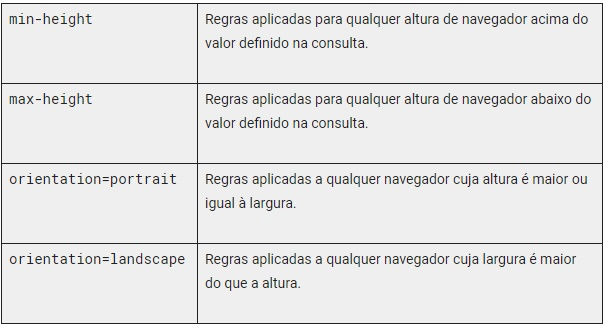
\includegraphics[width=15cm]{recursos/2.jpg}
\label{Media}
\caption{Media Query. Fonte: https://developers.google.com/web/fundamentals/design-and-ux/responsive/?hl=pt-br em 27/10/2017}
\end{figure}

Vejamos um exemplo:

\begin{figure}[!htb]
\centering
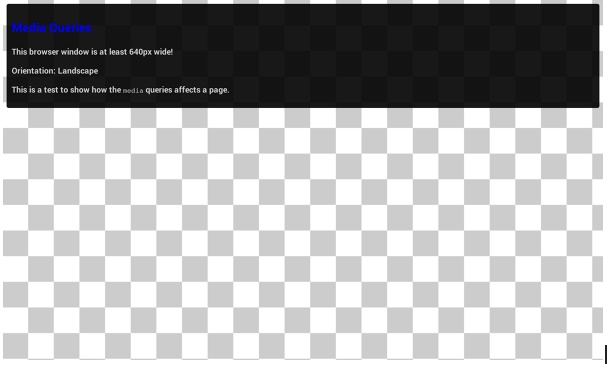
\includegraphics[width=15cm]{recursos/3.jpg}
\label{Media}
\caption{Media Query. Fonte: https://googlesamples.github.io/web-fundamentals/fundamentals/design-and-ux/responsive/media-queries.html em 27/10/2017}
\end{figure}

\subsection{Media Query} 
\lstinputlisting{recursos/exe3.html}

\begin{itemize}
\item Quando o navegador estiver entre 0 e 640 pixels de largura,  max-640px.css será aplicado.
\item Quando o navegador tiver entre 500 e 600 de largura, os estilos em @media serão aplicados.
\item Quando o navegador tiver 640 ou mais pixels de largura, min-640px.css será aplicado.
\item Quando a largura do navegador for maior do que sua altura, landscape.css será aplicado.
\item Quando a altura do navegador for maior do que sua largura, portrait.css será aplicado.
\end{itemize}


\section{Conclusão}
No desenvolvimento de aplicações web atualmente é imprescindível a utilização de layouts somente para navegador, visto que hoje o grande fluxo de acesso provém de dispositivos móveis. A utilização da meta tag viewport e  de mídias querys em layouts tornam-os mais flexíveis e adaptativos com fácil implementação e com ótimos resultados.

\section{Referências}
\begin{enumerate}

\item Google. \textbf{Google developers} Disponível em: $<$https://developers.google.com/web/fundamentals/design-and-ux/responsive/?hl=pt-br$>$. Acesso em: 27 de outubro de 2017.

\end{enumerate}

\end{document}